\documentclass[slidestop,compress,mathserif]{beamer}
\usepackage{fontspec,xunicode,xltxtra,beamerthemesplit}
\usepackage{graphicx}
\usepackage{color}
\usepackage{xcolor}
\usepackage{multicol}
\usepackage{animate}
\usepackage[labelsep=quad]{caption}[2011/11/10]
\usepackage{float}
\usepackage{picins}

\renewcommand{\figurename}{}

\graphicspath{{figures/}}

%以下是各种演示主题,定义幻灯片中的所有细节
%\usetheme{default}
%\usetheme{Berlin}%这个主题比较好
%\usetheme{Pittsburgh}
%\usetheme{Rochester}
\usetheme{Berkeley}%这种演示主题比较好
%\usetheme{Goettingen}
%\usetheme{Hannover}
%\usetheme{Marburg}
%\usetheme{PaloAlto}%这种演示主题比较好
%\usetheme{Antibes}
%\usetheme{Darmstadt}
%\usetheme{JuanLesPins}
%\usetheme{Montpellier}
%\usetheme{Singapore}
%\usetheme{Boadilla}
%\usetheme{Madrid}
%\usetheme{AnnArbor}
%\usetheme{CambridgeUS}
%\usetheme{Copenhagen}
%\usetheme{Warsaw}

%以下是各种外部主题,确定幻灯的显示式样
%\useoutertheme{infolines}
%\useoutertheme{miniframes}
%\useoutertheme[height=0.1\textwidth,width=0.15\textwidth,hideothersubsections]{sidebar}
%\useoutertheme{smoothbars}
%\useoutertheme{split}
%\useoutertheme{shadow}
%\useoutertheme{tree}
%\useoutertheme{smoothtree}
%\useoutertheme[height=0.5\textwidth]{sidebar}

%以下是各种内部主题
%\useinnertheme{default}
%\useinnertheme{circles}
%\useinnertheme{rectangles}
\useinnertheme[shadow]{rounded}

%以下是各种颜色主题
%\usecolortheme{default}
%\usecolortheme{albatross}
%\usecolortheme{beaver}
%\usecolortheme{beetle}
%\usecolortheme{crane}
%\usecolortheme{dolphin}
%\usecolortheme{dove}
%\usecolortheme{fly}
%\usecolortheme{lily}
%\usecolortheme{orchid}
%\usecolortheme{rose}
%\usecolortheme{seagull}
\usecolortheme{seahorse}
%\usecolortheme{sidebartab}
%\usecolortheme{structure}
%\usecolortheme{whale}
%\usecolortheme{wolverine}

%以下是各种字体主题
%\usefonttheme{default}
%\usefonttheme[onlymath]{serif}
%\usefonttheme{structurebold}
%\usefonttheme{structureitalicserif}
%\usefonttheme{structuresmallcapsserif}

\setsansfont[Mapping=tex-text, BoldFont={Microsoft YaHei Bold}]{Microsoft YaHei}

% 中文环境自动换行
\XeTeXlinebreaklocale "zh"  % 表示用中文的断行
\XeTeXlinebreakskip = 0pt plus 1pt % 多一点调整的空间

% 中文环境修正导航栏
\makeatletter
\setbeamertemplate{blocks}[rounded][shadow=true] 
\def\beamer@linkspace#1{
  \begin{pgfpicture}{0pt}{-1.5pt}{#1}{5.5pt}
    \pgfsetfillopacity{0}
    \pgftext[x=0pt,y=-1.5pt]{.}
    \pgftext[x=#1,y=5.5pt]{.}
  \end{pgfpicture}}
\makeatother

% 超链接高亮显示
\hypersetup{CJKbookmarks=true,
colorlinks=true,
citecolor=blue,
linkcolor=blue,
urlcolor=blue,
bookmarksopen=true,
breaklinks=true
}


% 幻灯片切换方式
%\transblindshorizontal 	% 水平百叶窗
%\transblindsvertical 		% 垂直百叶窗
%\transboxin				% 盒状收缩
%\transboxout				% 盒状展开
%\transdissolve				% 溶解
%\transglitter
%\transsplithorizontalin	% 上下向中央收缩
%\transsplitverticalin		% 垂直向中央收缩
%\transsplithorizontalout	% 上下向中央展开
%\transsplitverticalout		% 垂直向中央展开
%\transwipe					% 从下抽出


\title{2002年图灵奖~\\~公钥密码学~\\~RSA加密算法}
\author{刘正~~徐小奇}
\date{\today}
%\institute{同济大学电信学院}

\logo{\color{blue!50}\scalebox{2}{{
\includegraphics[height=0.8cm]{logo.jpg}\vspace{220pt}}}}

% 设定frametitle居中
\makeatletter 
\long\def\beamer@@frametitle[#1]#2{% 
  \beamer@ifempty{#2}{}{% 
    \gdef\insertframetitle{\centering{#2\ifnum\beamer@autobreakcount>0\relax{}\space\usebeamertemplate*{frametitle continuation}\fi}}% 
  \gdef\beamer@frametitle{#2}% 
  \gdef\beamer@shortframetitle{#1}% 
}% 
} 
\makeatother


\begin{document}

\frame{\titlepage}

\section{RSA加密算法}

\begin{frame}
  \transdissolve
  \frametitle{加密的历史}
  
  \begin{block}<+->{1976年以前,所有的加密方法都是同一种模式:}
    \begin{itemize}[<+->]
        \item 甲方选择某一种加密规则,对信息进行加密;
        \item 乙方使用同一种规则,对信息进行解密。
    \end{itemize}
  \end{block}

\end{frame}

\begin{frame}
  \frametitle{加密的历史}
  
  \begin{block}{1976年以前,所有的加密方法都是同一种模式:}
    \begin{itemize}
        \item 甲方选择某一种加密规则,对信息进行加密;
        \item 乙方使用同一种规则,对信息进行解密。
    \end{itemize}
  \end{block}
  ~\\[0.6cm]

~ ~ ~ ~由于加密和解密使用同样规则(简称"密钥"),这被称为"对称加密算法"(Symmetric-key algorithm)。

~ ~ ~ ~这种加密模式有一个最大弱点:甲方必须把加密规则告诉乙方,否则无法解密。保存和传递密钥,就成了最头疼的问题。
\end{frame}

\subsection{\hfill 凯撒密码}
\begin{frame}
  \frametitle{凯撒密码}
\end{frame}
\begin{frame}
  \frametitle{凯撒密码}
  ~~~~字母之间的替换---它的几个变种:换字式密码(破解的方法可以使用字符频数分析法)、转置式密码、多表替换密码(先分组后凯撒加密)
\end{frame}
\begin{frame}
\transboxout
  \frametitle{凯撒密码}
  ~~~~字母之间的替换---它的几个变种:换字式密码(破解的方法可以使用字符频数分析法)、转置式密码、多表替换密码(先分组后凯撒加密)
  \begin{figure}
    \centering
    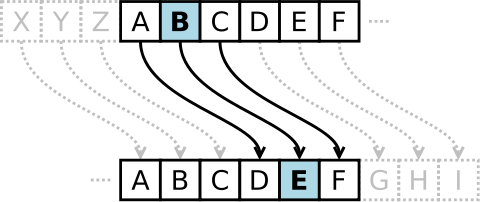
\includegraphics[width=5cm]{Caesar3.png}
  \end{figure}
\end{frame}


%\begin{frame}
%  \frametitle{凯撒密码}
%  \begin{itemize}[<+->]
%    \item{明文字母表:}ABCDEFGHIJKLMNOPQRSTUVWXYZ
%    \item{密文字母表:}DEFGHIJKLMNOPQRSTUVWXYZABC
%    \item{明文:}THE QUICK BROWN FOX JUMPS OVER THE LAZY DOG
%    \item{密文:}WKH TXLFN EURZQ IRA MXPSV RYHU WKH ODCB GRJ
%    \end{itemize}
%
%\end{frame}
%\begin{frame}
%  \frametitle{凯撒密码}
%  \begin{itemize}
%    \item{明文字母表:}ABCDEFGHIJKLMNOPQRSTUVWXYZ
%    \item{密文字母表:}DEFGHIJKLMNOPQRSTUVWXYZABC
%    \item{明文:}THE QUICK BROWN FOX JUMPS OVER THE LAZY DOG
%    \item{密文:}WKH TXLFN EURZQ IRA MXPSV RYHU WKH ODCB GRJ
%    \end{itemize}
%  恺撒密码的加密、解密方法还能够通过同余的数学方法进行计算。首先将字母用数字代替,A=0,B=1,\ldots,Z=25。此时偏移量为n的加密方法即为:
%
%  \begin{equation}
%    E_n=(x+n) ~mod~ 26
%  \end{equation}
%  解密就是:
%  \begin{equation}
%    D_n=(x-n) ~mod~ 26
%  \end{equation}
%
%\end{frame}


\subsection{\hfill 栅栏密码}
\begin{frame}
  \frametitle{栅栏密码}
\end{frame}
\begin{frame}
  \transwipe
  \frametitle{栅栏密码}
%加密的明文分成N个一组,然后把每组的第1个字连起来,形成一段无规律的话
  ~\\[1.6cm]
    ~~~~所谓栅栏密码,就是把要加密的明文分成N个一组,然后把每组的第1个字连起来,形成一段无规律的话。 不过栅栏密码本身有一个潜规则,就是组成栅栏的字母一般不会太多。(一般不超过30个,也就是一、两句话)
\end{frame}

%\subsection{\hfill 维基尼亚密码}
%\begin{frame}
%  \frametitle{维基尼亚密码}
%引入密钥 对抗字频统计既同一个密文字符对应该的明文不一定是相同的)
%\end{frame}
\subsection{\hfill RSA加密算法}
\begin{frame}
  \frametitle{RSA加密算法}
\end{frame}
\begin{frame}
  \transsplitverticalin
  \frametitle{RSA加密算法}
 ~ ~ ~ ~RSA加密算法是一种非对称加密算法。在公开密钥加密和电子商业中RSA被广泛使用。

~ ~ ~ ~ RSA是1977年由罗纳德·李维斯特(Ron Rivest)、阿迪·萨莫尔(Adi Shamir)和伦纳德·阿德曼(Leonard Adleman)一起提出的。当时他们三人都在麻省理工学院工作。RSA就是他们三人姓氏开头字母拼在一起组成的。

~ ~ ~ ~ 1973年,在英国政府通讯总部工作的数学家克利福德·柯克斯(Clifford Cocks)在一个内部文件中提出了一个相同的算法,但他的发现被列入机密,一直到1997年才被发表。

\end{frame}


\begin{frame}
  \transboxout
  \frametitle{RSA加密算法}
  \begin{center}
    \begin{figure}
      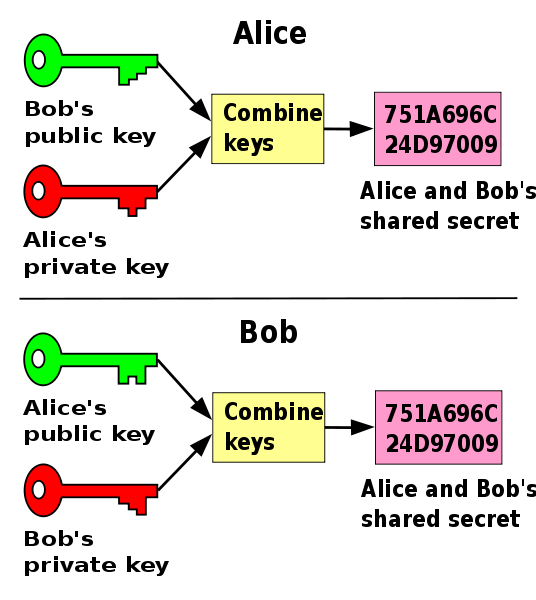
\includegraphics[width=6cm]{Publickeysharedsecret.svg.png}
    \end{figure}
  \end{center}
\end{frame}

\section{获奖者生平}
% http://www.techcn.com.cn/index.php?doc-view-131079.html#1

\begin{frame}
  \frametitle{获奖啦}
  \parpic(11cm,6cm){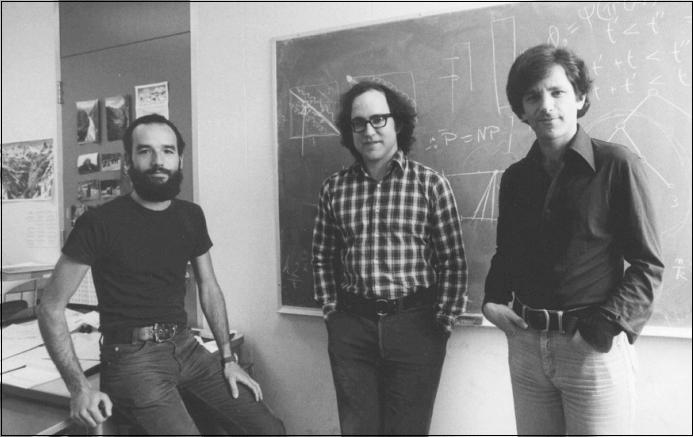
\includegraphics[width=9cm]{3peoples}}

\end{frame}

\begin{frame}
  \transboxout
  \frametitle{获奖啦}
  \parpic(11cm,6cm){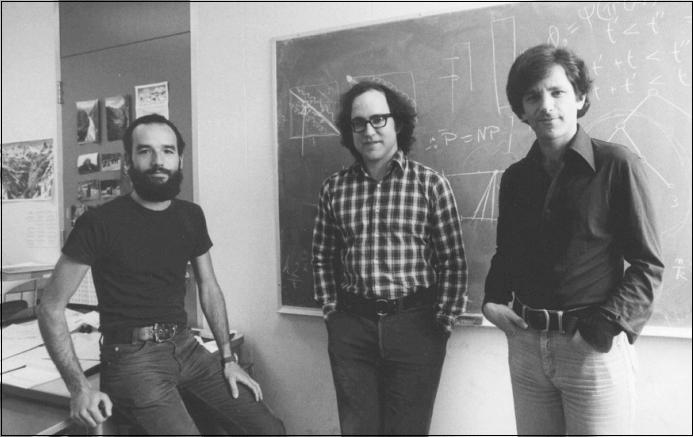
\includegraphics[width=9cm]{3peoples}}
  \parpic(11cm,6cm){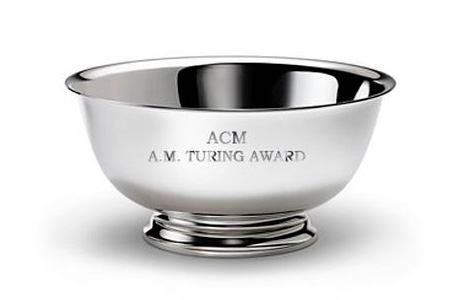
\includegraphics[width=5cm]{turing}}


\end{frame}

\subsection{\hfill Cocks}
\begin{frame}
  \frametitle{Clifford Cocks}
  
  \begin{multicols}{2}
    \begin{figure}
      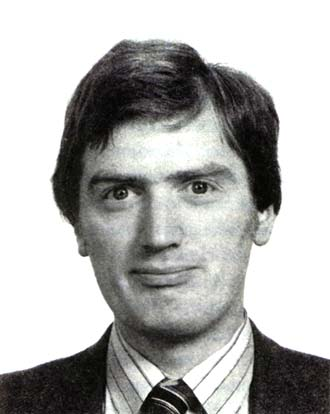
\includegraphics[width=3cm]{Cocks.jpg}
    \end{figure}
    Clifford Christopher Cocks出生于1950年12月28日,是英国数学家,密码学家,任职于英国国家通讯总部(GCHQ).
    
    He invented the widely used encryption algorithm now commonly known as RSA, about three years before it was independently developed by Rivest, Shamir, and Adleman at MIT. He has not been generally recognised for this achievement because his work was classified information, and therefore not released to the public at the time.

    
  \end{multicols}
  
\end{frame}

\subsection{\hfill Rivest}
\begin{frame}
  \frametitle{Ronald L. Rivest}
  \begin{multicols}{2}
    \begin{figure}
      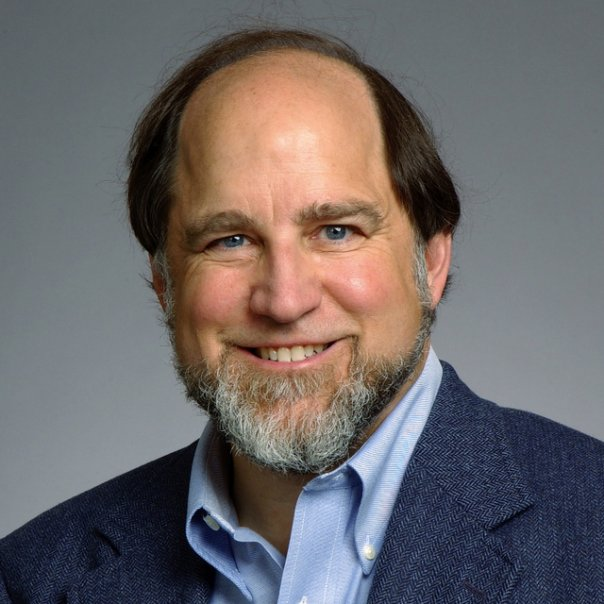
\includegraphics[width=3cm]{rivest_photo.jpg}
      \caption{1947, Schenectady, New York, USA}
    \end{figure}
    
  \end{multicols}
  
\end{frame}

\subsection{\hfill Shamir}

% EDUCATION
\begin{frame}
  \frametitle{Adi Shamir}
  \begin{multicols}{2}
    \begin{minipage}[c]{0.5\textwidth}
      \begin{figure}[H]
        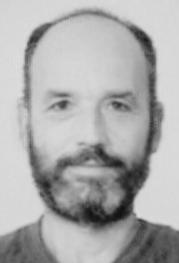
\includegraphics[width=3cm]{Shamir.jpg}
        \caption{July 6, 1952, Tel Aviv, Israel}
      \end{figure}
    \end{minipage}

    BSc (Mathematics, Tel Aviv University, 1973); 
   
    ~\\ 
    
    MSc (Computer Science, Weizmann Institute, Israel, 1975); 
    
    ~\\

    PhD (Computer Science, Weizmann Institute, Israel, 1977)    
  \end{multicols}
  
\end{frame}
% EXPERIENCE
\begin{frame}
  \frametitle{Adi Shamir}
  \begin{multicols}{2}
    \begin{minipage}[c]{0.5\textwidth}
      \begin{figure}[H]
        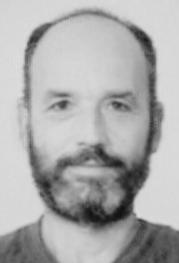
\includegraphics[width=3cm]{Shamir.jpg}
        \caption{July 6, 1952, Tel Aviv, Israel}
      \end{figure}
    \end{minipage}

     \footnotesize
    Post doctorate position, Warwick University, England (1976); 
    
    Instructor, Department of Mathematics, MIT (1977-1978); 
    
    Assistant Professor Department of Mathematics, MIT (1978-1980);
    
    Associate Professor at Department of Applied Mathematics, Weizmann Institute of Science, Rehovot, Israel (1980-1984);
    
    Professor, Department of Applied Mathematics, The Weizmann Institute of Science, Rehovot, Israel(1984 onward) Invited Professor, École Normale Suprieure, Paris (2006 onward).
  \end{multicols}
  
\end{frame}
% HONORS & AWARDS
\begin{frame}
  \frametitle{Adi Shamir}
  \begin{multicols}{2}
    \begin{minipage}[c]{0.5\textwidth}
      \begin{figure}[H]
        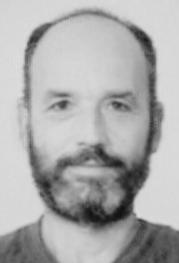
\includegraphics[width=3cm]{Shamir.jpg}
        \caption{July 6, 1952, Tel Aviv, Israel}
      \end{figure}
    \end{minipage}
    \footnotesize
    Israel Prize (2008); 
    
    ACM Turing Award (2002 – jointly with R. Rivest and L. Adleman);
    
    IEEE Koji Kobayashi Computers and Communications Award (2000); 
    
    ACM Paris Kanellakis Theory and Practice Award (1996 – again jointly with others for RSA); 
    
    UAP Scientific Prize (1990); 
    
    IEEE WRG Baker Award (1986); 
    
    Vatican Pontifical Academy PIUS XI Gold Medal (1992); 
    
    Israel Mathematical Society Erdos Prize (1983); 
    
    Elected to the Israeli Academy of Science (1998); 
    
    Fellow, International Association of Cryptographic Research (2004); 
    
    Elected to the US National Academy of Sciences (2005); 
    
    Honorary Doctorates from École Normale Suprieure (2003) and the University of Waterloo (2009).    
  \end{multicols}
  
\end{frame}
\begin{frame}
  \frametitle{Adi Shamir}
  \begin{multicols}{2}
    \begin{minipage}[c]{0.5\textwidth}
      \begin{figure}[H]
        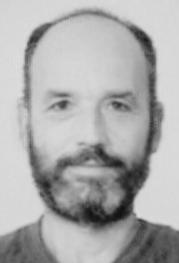
\includegraphics[width=3cm]{Shamir.jpg}
        \caption{July 6, 1952, Tel Aviv, Israel}
      \end{figure}
    \end{minipage}

  \end{multicols}
  
\end{frame}
\subsection{\hfill Adleman}
\begin{frame}
  \frametitle{Leonard M. Adleman}
  \begin{multicols}{2}
    \begin{figure}
      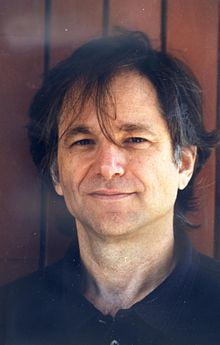
\includegraphics[width=3cm]{Adleman.jpg}
    \end{figure}
    
  \end{multicols}

\end{frame}





\section{八卦环节}
\begin{frame}
  \transblindsvertical
  \frametitle{八卦环节}
 ~~~~当年第一个公开密钥算法是背包算法,其发明者Ralph Merkle对这个算法极有信心,确信这个算法不可能被攻破,所以他悬赏100美元奖金给破解算法的人。Adi Shamir迅速破解了该算法,并领走了奖金。Shamir就是RSA算法的发明人之一。

 ~~~~但Merkle并没有气馁,他又加强了算法,并悬赏1000美元奖金,给破解新算法的人。结果Ronald Rivest也迅速地破解了该算法,并领走了奖金。Rivest是RSA算法的另一个发明人。

 ~~~~于是,Merkle终于没有胆量尝试第三次悬赏,于是RSA的最后一个作者Leonard Adleman也就没有机会成为万元户了。(按照规律,Merkle如果要悬赏,应该是10000美金了。)
\end{frame}








\begin{frame}
\frametitle{我是中文} 
%\framesubtitle{\centerline{subtext}} 
\animate<3-6>% 自动逐步显示
\begin{itemize}[<+->]
\item one
\item two
\item three
\item four
\item five
\item six
\end{itemize}

刘正 徐小奇 e
\end{frame}


















\end{document}
